\begin{document}
\section{Sprint 1}

\textbf{Goals for Sprint 1}\\\\
    Intake:
    \begin{itemize}
        \item Design and CAD new intake
        \item Order new wheels for intake
        \item Build intake
    \end{itemize}
    Outtake:
    \begin{itemize}
        \item CAD virtual four bar linkage (VFBL) with slides
        \item Design and CAD claw (design meeting)
        \item Order parts
    \end{itemize}
    3D printing
    \begin{itemize}
        \item Phone mount
        \item Battery mount
    \end{itemize}
\vspace{1in}
\meetingnotes{9/18/19 6:00pm - 9:00pm}{Sprint 1 Meeting}{Dominik, Josh, Julia, Liana, Michael, Oliver, Ori, Rachel, Sarah}{
    General problems & The entire design was pretty janky, which is what we expected from building a robot in such a short amount of time. The robot actually doesn't currently fit in the 18" box because the arm gets in the way of the intake. We need to make a phone mount and a battery mount, and re-engineer most of the robot components.\\\\
    
    Arm design & Our general idea works well but needs to be redone slightly, is pretty janky but could be redone to work well. We will probably put the arm on a drawer slide lift to make it easier to stack the Stones higher. \\\\
    
    Wheeled intake & Works pretty well but we are going to get different wheels.\\\\
    Next steps & Autonomous code, test the robot with the field, potentially resign the arm depending on tests, redo everything to make everything more stable and reliable, design and print phone/battery mounts.\\\\
    Team processes & We've agreed on using a system with sprints and tasks for our design process. At the beginning of each 2-week sprint, we will discuss the tasks we want to accomplish in the sprint, and assign people to each task in groups of at least 2 per task, but individuals can do individual assignments within the tasks. We will only CAD when we have all agreed on a design.
}
%virtual four bar linkage
\practicenotes{9/18/19 6:00pm - 9:00pm}{Sprint 1 - Practice}{Dominik, Josh, Julia, Liana, Michael, Oliver, Ori, Rachel, Sarah}{
    
    Design and CAD\\\\
    We had a full-team design meeting to discuss all the components of the robot that we are changing.\\\\
    \textit{Outtake design meeting:} We will have 2 pairs of drawer slides to mount the virtual four bar linkage on. We need to keep the robot under 14" to go under the Skybridge. We can get either 8" or 12" slides, but the 12" slides would need to be mounted on the side of the drive train, whereas the 8" could be mounted on top of the chassis.\\\\
    \textit{Intake design meeting:} We can add a ramp to the intake and have the Stones end up more in the middle of the robot and slightly elevated to make it easier to pick up, and then the arm won't get in the way of the intake.\\\\
    \textit{Claw:} We could have a claw that rotates, but we would have to add another servo for this which adds weight to the end of the arm. We would also need to figure out how to have the Stone not hit the bars that hold up the VFBL. We are also changing the design of the claw to hold onto only one side of the Stone and one of the studs instead of holding both sides of the Stone.\\\\
    Written by: Rachel
}

\practicenotes{9/20/19 6:00pm - 9:00pm}{Sprint 1 - Practice}{Dominik, Josh, Julia, Liana, Michael, Oliver, Ori, Rachel, Sarah}{
    Robot test\\\\
    We immediately realized that the Stones were bigger than the cardboard one we had made to test, and the Stones didn't really fit in our current claw. This is fine, since we are planning on making a new one anyway. There was also a bit of drift when we drove sideways with the mecanum wheels, so we need to figure out what caused that. We also need to make sure our next design will keep the Stone completely aligned once we intake it, since on the current robot, there is too much space and the Stones turn a bit sideways, which makes it hard for the claw to pick it up.\\\\
    Written by: Rachel
    \newBox
    CAD and Design\\\\
    Oliver is CADing a new intake. We decided on using small stealth wheels instead of compliant wheels because the intake itself is already compliant because of the springs.\\\\
    Written by: Rachel
}
\practicenotes{9/23/2019 3:30pm - 9:00pm}{Sprint 1 - Practice}{Dominik, Josh, Julia, Liana, Michael, Oliver, Ori, Rachel, Sarah}{
    Meeting\\\\
    We had a meeting at the beginning of practice to discuss how we were going to function as a team as well as catching people up who had just recently joined the team. We also re-discussed the roles for a Coach and discussed what we as team members have to do to be certain that everyone on the team would remain happy with each other.\\\\
    Written by: Sarah
    \newBox
    Logistics\\\\
    We spent today doing inventory on all of the pieces we had at Ori's house so we knew which parts we had from the club and which parts were the team's and Michael's. \\\\
    Written by: Sarah
    \newBox
    CAD and Design\\\\
    Oliver continued to work on the new intake for the robot. \\\\
    Written by: Sarah
}

\practicenotes{9/25/2019 6:00pm - 9:00pm}{Sprint 1 - Practice}{Dominik, Josh, Julia, Liana, Michael, Ori, Rachel, Sarah}{
    Logistics\\\\
    Ori helped other club members with organizing all of the parts in the club. They recorded every supply the club had onto a spreadsheet. This helped the club to be more organized and aware of what pieces we have and helps teams be able to figure out if they need to order a new part for their robot or if they can take them from the club supplies.\\\\
    Written by: Dominik \& Julia
    \newBox
    Notebook\\\\
    Rachel taught Dominik and Julia the basics of how to use Overleaf to write journal entries for practices, meetings, and competitions. This included teaching them the basics of inserting the photos and all of the commands to have the text wrap the photos and other things. Rachel also taught them the basics of the main in Overleaf and showed them the different formats. They now are ready to assist in writing the Engineering Notebook entries and are super excited! \\\\
    Written by: Dominik \& Julia
}

\practicenotes{9/30/19 3:30pm - 6:30pm}{Sprint 1 - Practice}{Dominik, Julia, Ori, Rachel, Sarah}{
    CAD and Design\\\\
    Ori is finalizing the design for the lift and the arm so that we can order parts.\\
    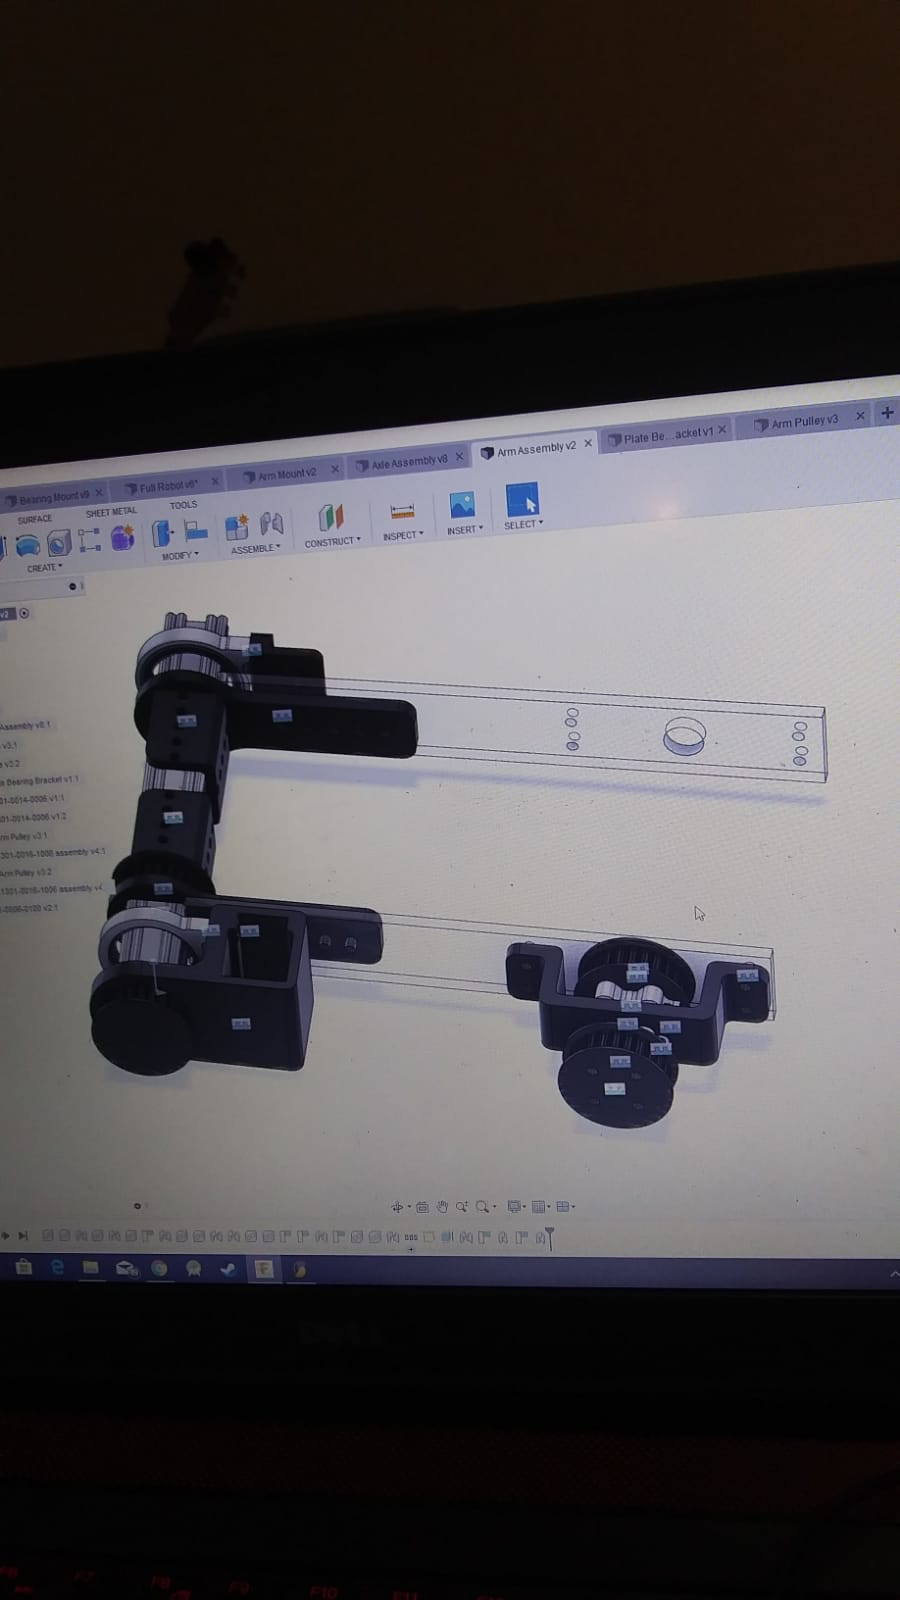
\includegraphics[width=.25\textwidth]{Images/10-1CADarm.png}\\
    Written by: Rachel
    \newBox
    Programming\\\\
    Michael is working on motion-profiling, and working on how to implement Road Runner. We are also considering making our own motion-profiling program.\\\\
    Written by: Rachel
}

\practicenotes{10/2/19 6:00pm - 9:00pm}{Sprint 1 - Practice}{Dominik, Josh, Julia, Liana, Michael, Ori, Rachel, Sarah}{
    Notebook\\\\
    Julia and Dominik are very excited to learn more notebook, and have made a plan for Rachel to teach them a few things.\\\\
    Written by: Julia
    \newBox
    Programming\\\\
    Michael and Josh are working hard on their code. However, they need to have a physical robot before they can fully finish it (of course), which is another reason why we really need to finish ordering all the parts we need.\\\\
    Written by: Julia
    \newBox
    Logistics\\\\
    The club decided to have an outreach meeting so that both students and parents could come to share their ideas regarding what different type of outreach and connect we should do. Julia and Sarah decided to attend this meeting a help propose and compose a list of different ideas the club wanted to do. We were fortunate to have been joined by 3 parents of members in the club who brought additional good ideas to the table. The list of connect ideas consisted of a lot of companies we wanted to try to visit sometime. Our composed Outreach list consisted of a lot of schools where we could show and educate both younger and older people about robotics as well as other locations like the local library.\\\\
    Written by: Sarah
}
\practicenotes{10/4/19 6:00pm - 9:00pm}{Sprint 1 - Practice}{Dominik, Julia, Liana, Michael, Ori, Rachel, Sarah}{
    Logistics\\\\
    The club had not yet finished auditing all of the club and team belongings so Sarah helped some other members of the club finish the auditing of the club pieces and the 7776 pieces. The other members of the club worked on cleaning out the dark room and organizing how things were set up in the room to make it work best for all 4 teams. After, the team tried to set up the field but unfortunately we ran out of time.\\\\
    Written by: Sarah
    \newBox
    Programming\\\\
    Michael wanted to test some of the code he had written for the season so he decided to take off the intake and the outtake of the robot so it could  be tested without things in the way. He then took the robot home.\\\\
    Written by: Sarah
}
\practicenotes{10/7/19 3:30pm - 8:00pm}{Sprint 1 - Practice}{Dominik, Julia, Liana, Ori, Rachel, Sarah}{
    Building\\\\
    We received all of the parts that we ordered except for the Misumi drawer slides, so we can build the new intake. Julia, Sarah and Dominik are working on disassembling the RI3D bot other than the drivetrain. Ori started building the structure for the slides so that we can assemble the lift when we get the slides. We are 3D printing brackets to attach to the box tube that will be part of the lift. He also assembled the rotating axle for the new arm. We worked on making the odometry pods: Sarah added ball bearings and Liana put together the encoders for the pods and attached them.
    \\\\
    We will be able to make the new intake after we 3D print the enclosures for the intake wheels, which will take awhile. Hopefully we will have these printed before Wednesday.
    %new robot CAD
    \\\\
    Written by: Rachel
    \newBox
    Notebook\\\\
    Rachel worked on getting rid of errors in Overleaf and eliminated half of the error we had. The remaining errors don't affect the compilation or layout of the notebook.\\\\
    Written by: Rachel
}

\practicenotes{10/9/19 6:00pm - 9:00pm}{Sprint 1 - Practice}{Dominik, Josh, Julia, Liana, Michael, Oliver, Ori, Rachel, Sarah}{
    Logistics\\\\
    Our team finished assembling the field for the club. Rachel and Ori also held a meeting with other experienced members of the club and one of the club's general managers to discuss forming a student leadership council, which will start meeting next week. This will improve communication between teams and coaches.
    Written by: Rachel
    \newBox
    CAD and Design\\\\
    We are 3D printing the intake mounts at Ori's house so that we can build the intake next practice. We also printed a mount for the gearbox that will raise and lower the lift.\\\\
    Written by: Rachel
    %CAD of the pieces
}

\practicenotes{10/11/19 1:00pm - 6:00pm}{Sprint 1 - Practice}{Dominik, Julia, Liana, Oliver, Ori, Rachel, Sarah}{
    CAD and Design\\\\
    Oliver worked on new CAD designs and tried to come up with new ideas for the robot.\\\\
    Written by: Julia
    \newBox
    
    \begin{wrapfigure}{r}{.45\textwidth}
        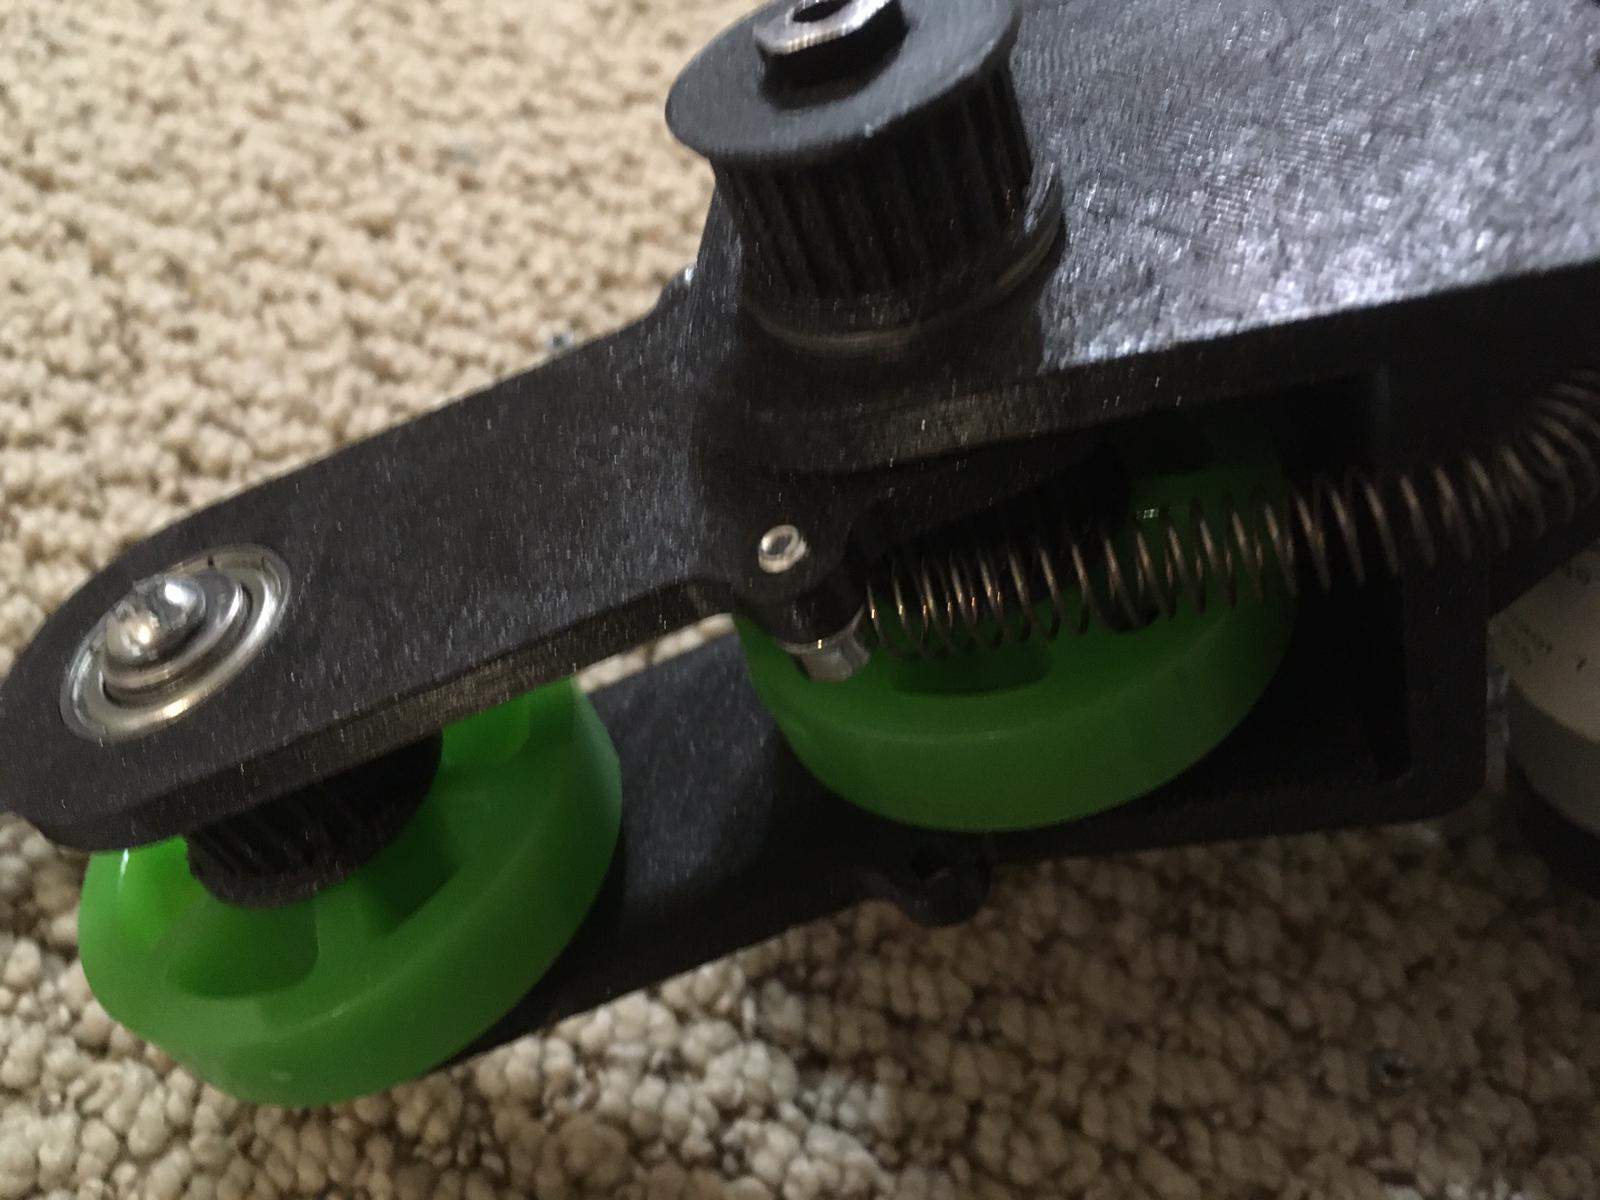
\includegraphics[width=.2\textwidth]{Images/10-11Intake.png}
        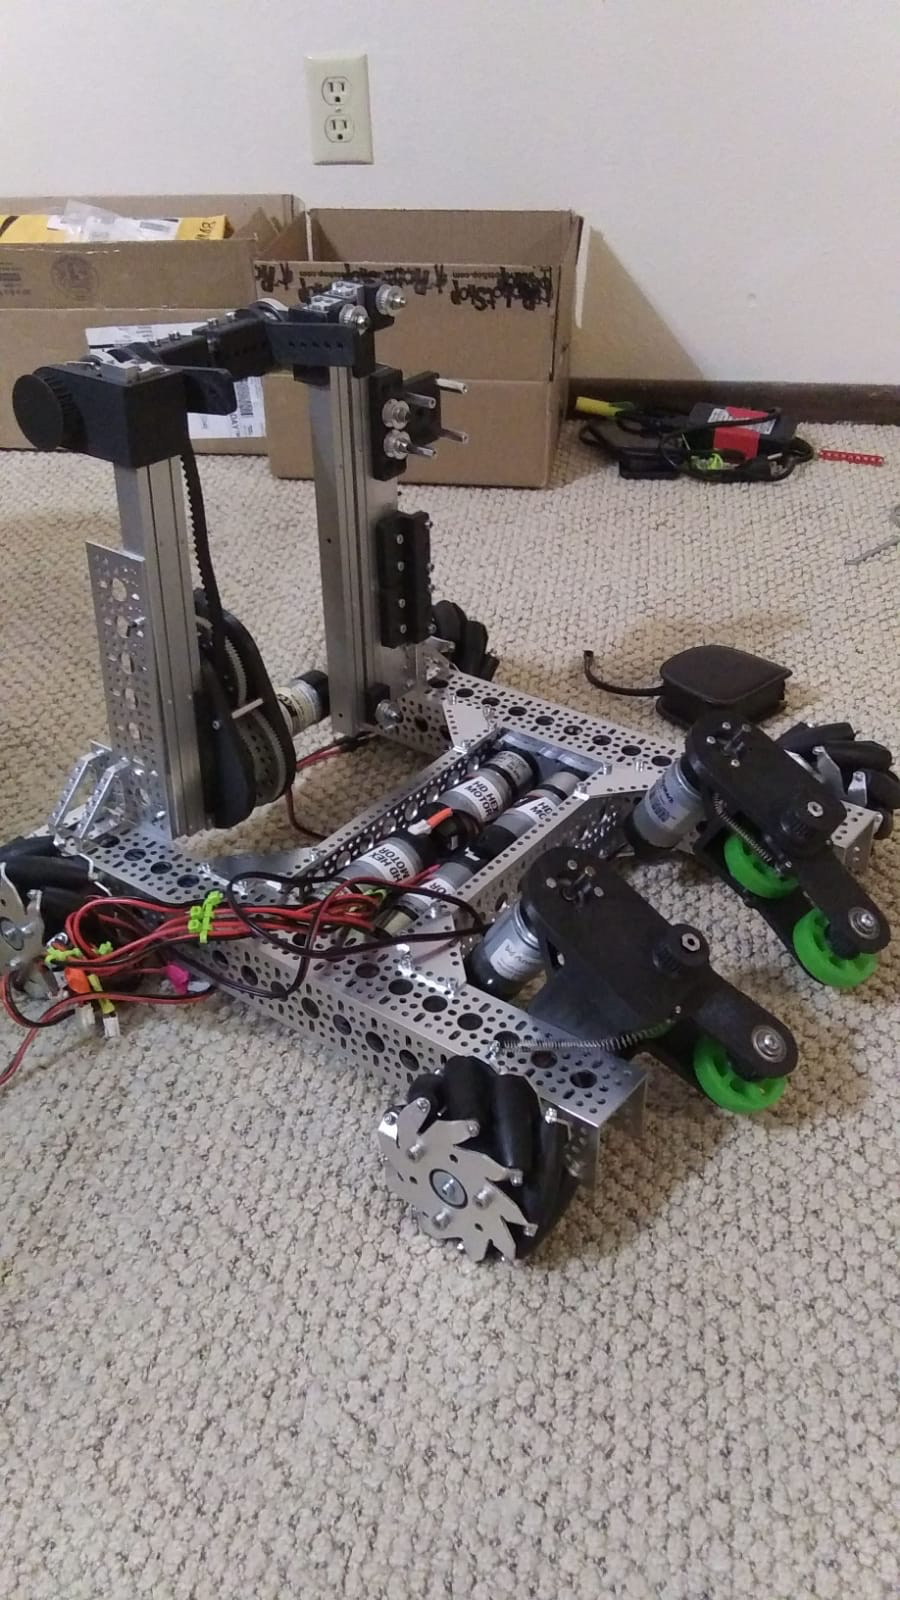
\includegraphics[width=.2\textwidth]{Images/10-11Robot.png}
    \end{wrapfigure}
    Build Team A    \\\\
    Oliver and Ori assembled the twin components of the intake\\ and mounted them to the front of the robot. The intakes use\\ 2 2-inch compliant wheels on each side powered by 3.7:1 motors.\\\\\\\\\\\\\\\\\\\\
    Written by: Rachel
    
    \newBox
    Build Team B\\
    \begin{wrapfigure}{l}{.45\textwidth}
        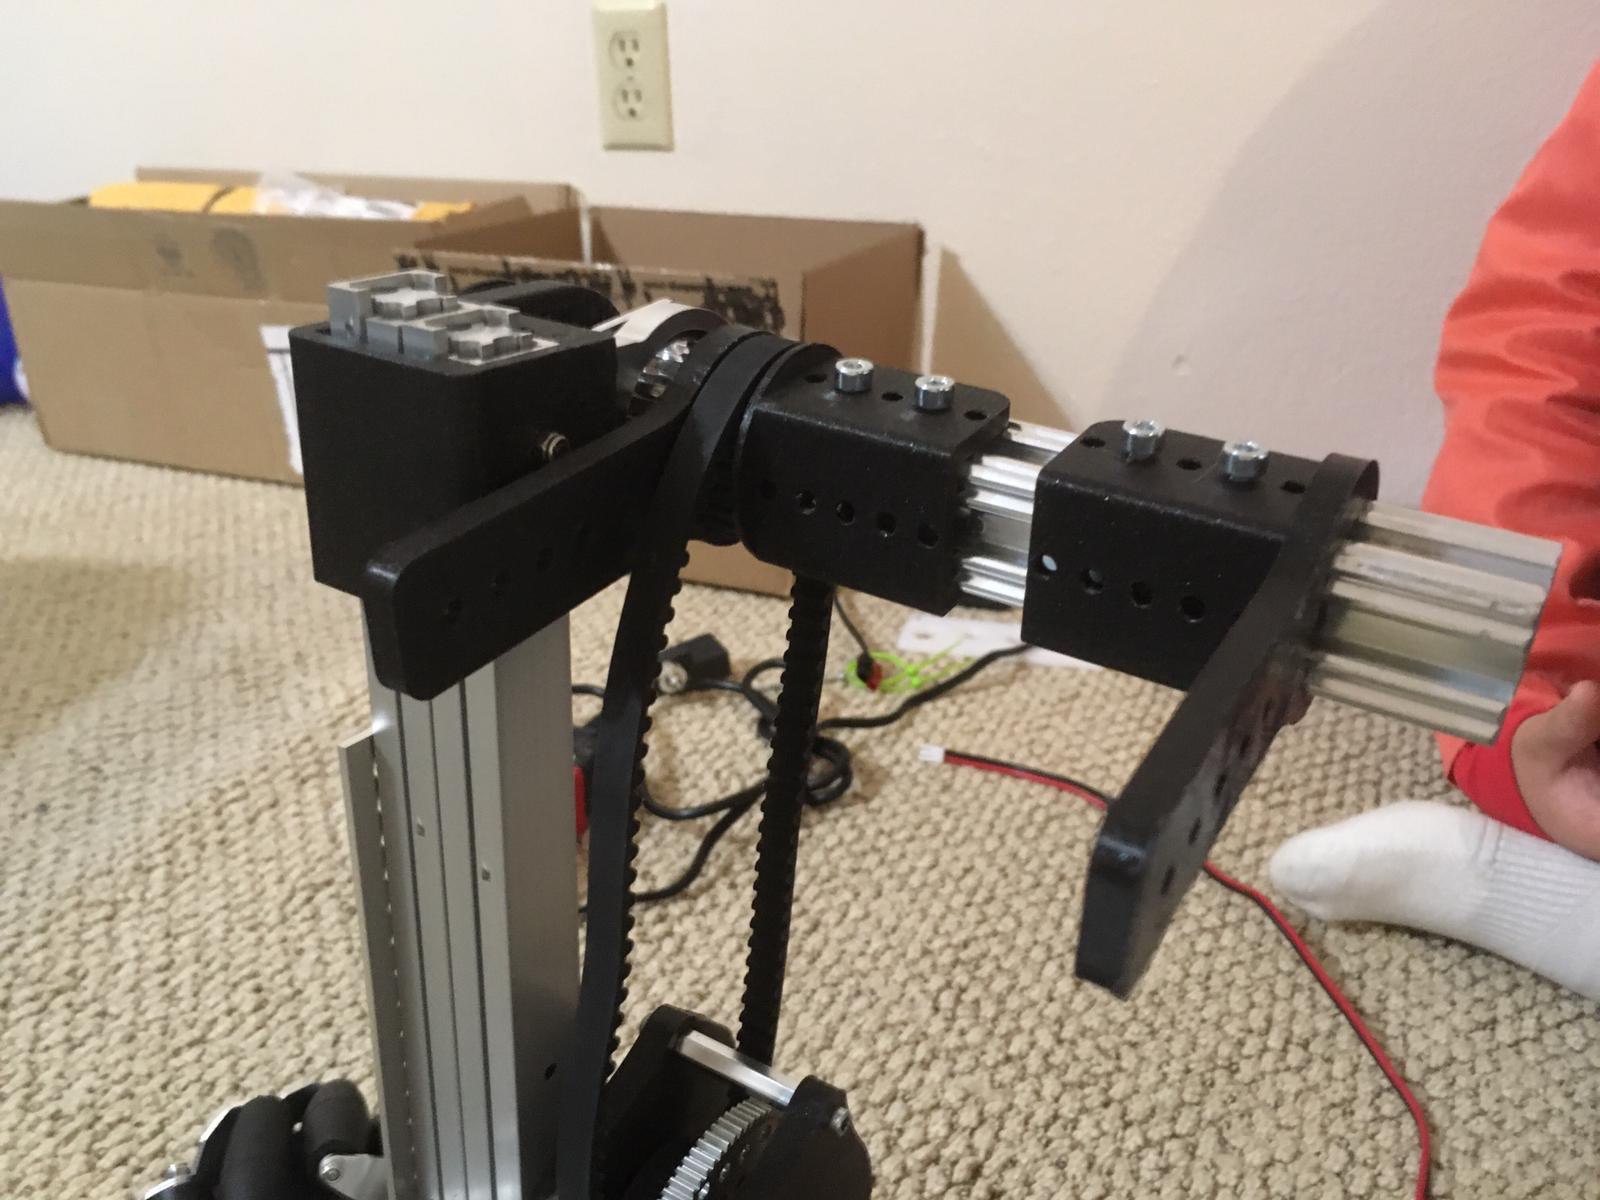
\includegraphics[width=.2\textwidth]{Images/10-11V4BJ.png}
        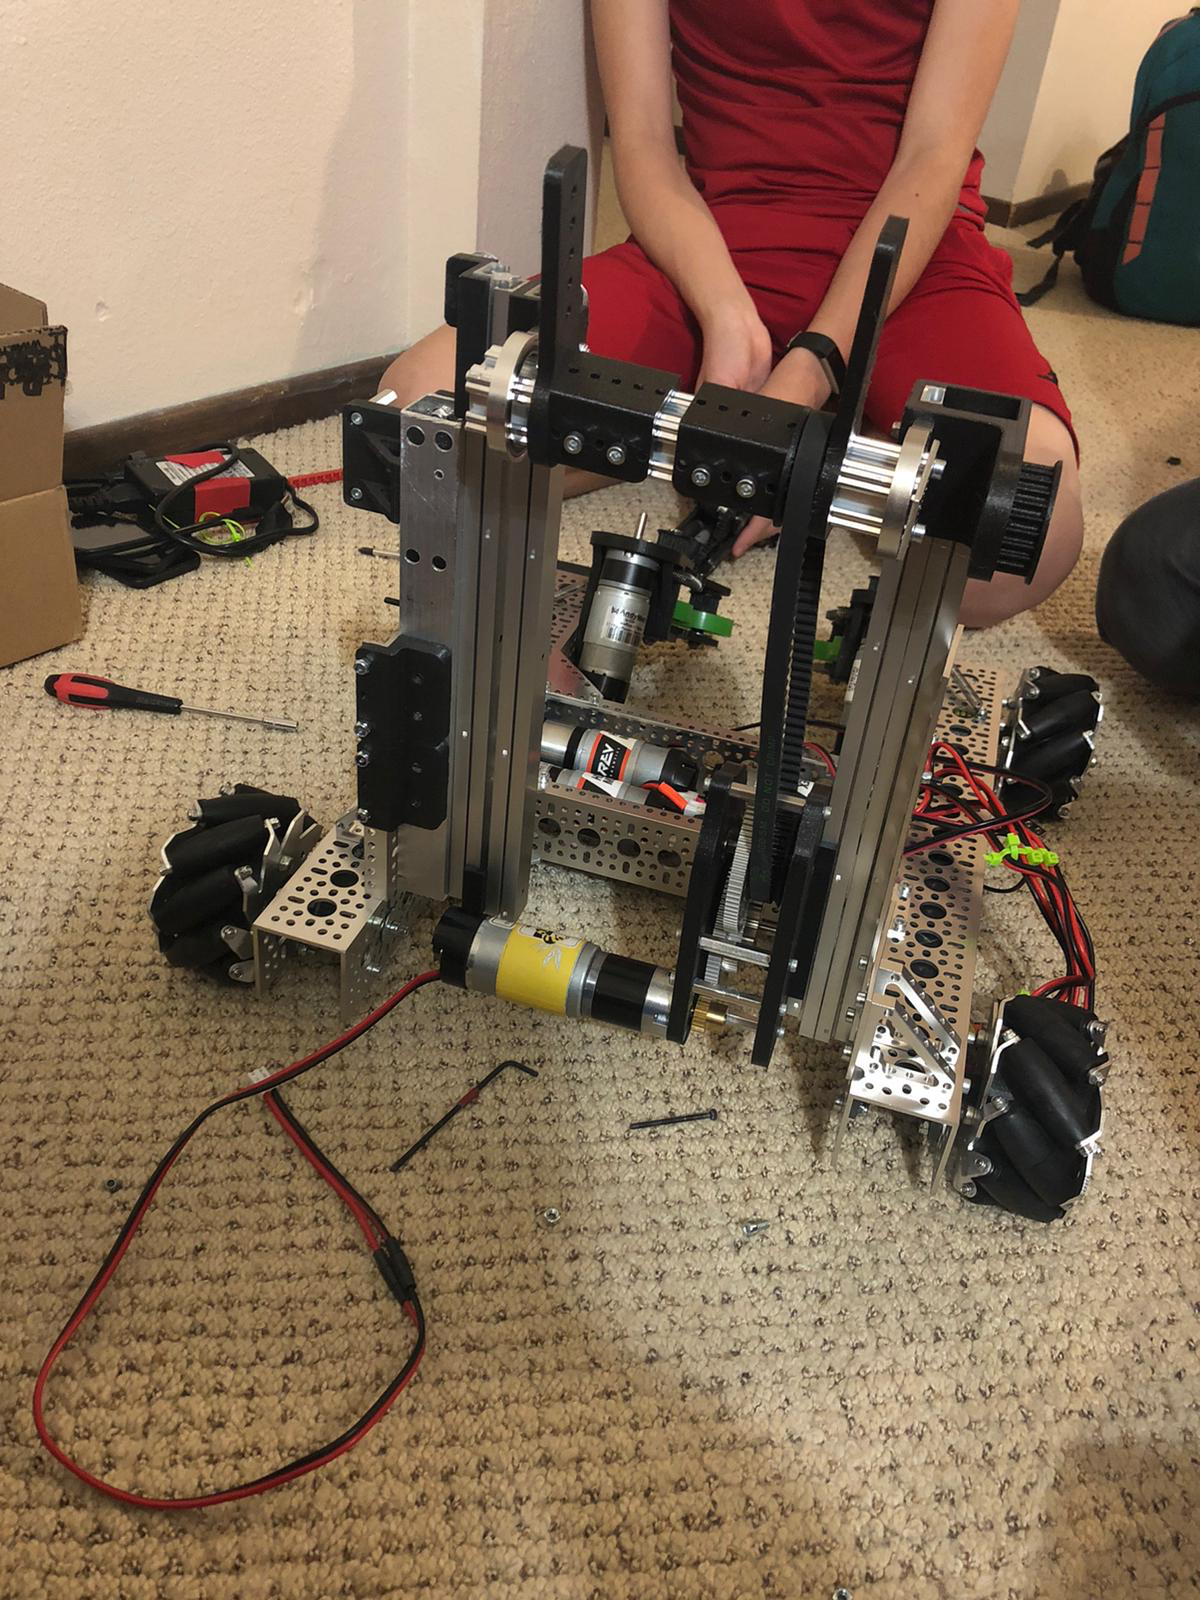
\includegraphics[width=.2\textwidth]{Images/10-11Robot2.png}
    \end{wrapfigure}
    Julia and Oliver drilled holes into the drawer slides so that each side of the lift would have 2 slides. Sarah and Dominik are assembling the base of the slide lift and attaching the slides to the boxtube. Dominik attached the slide to the 3D printed gearbox parts. Ori assembled the slides. \\\\\\\\
    \hspace{5in}
    Written by: Rachel
    \newBox
    Notebook\\\\
    Worked on a way to put either colors and/or section titles in the margins instead of in the header because it will be easier to navigate the notebook.\\\\
    Written by: Rachel
}

\practicenotes{10/14/19 3:30pm - 8:00pm}{Sprint 1 - Practice}{Dominik, Josh, Julia, Liana, Michael, Oliver, Ori, Rachel, Sarah}{
    CAD and Design\\\\
    Oliver is finishing a CAD model for the claw, which we will build later in the week.\\\\ %add cad renders
    Written by: Rachel
    \newBox
    Build Team A\\\\
    Liana and Dominik remade the slides because one side was mounted too high and wouldn't fit under the Skybridge (14"). The height difference also made the joint for the virtual 4-bar linkage uneven and not parallel to the ground. They drilled new holes in the boxtube and remounted the slides to be at the correct height.\\\\
    Written by: Rachel
    \newBox
    Build Team B\\\\
    Michael, Sarah, and Oliver worked on mounting the odometry pods. Liana cut down the axles and the pods are being mounted to the sides of the chassis.\\\\
    Written by: Rachel
}

\practicenotes{10/16/19 6:00pm - 9:00pm}{Sprint 1 - Practice}{Dominik, Josh, Julia, Liana, Michael, Oliver, Ori, Rachel, Sarah}{
    CAD and Design\\\\
    Oliver finished the CAD for the claw. However in a team design meeting we discussed having a different outtake mechanism. Instead of grabbing the side of the Stone facing the back of the robot, the claw will now grab the side facing the front of the robot. This change was made so that the Stone can clear the axle of the arm when we move the Stone to the other side of the bot.\\\\
    Written by: Julia
    \newBox
    Programming\\\\
    Josh and Michael explored the possibility of using Vuforia to detect the Skystones. Josh and Michael also made a plan for an early autonomous\\\\
    Written by: Julia
}

\practicenotes{10/18/19 6:00pm - 9:00pm}{Sprint 1 - Practice}{Josh, Michael}{
    Programming\\\\
    Josh or Michael planned out an early autonomous and continued to explore using Vuforia to detect the Skystones. Josh and Michael also spent a lot of time helping the member of 7776, 9231 and 11625 with their software.\\\\
    Written by: Sarah
}
\practicenotes{10/19/19 2:30pm - 4:30pm}{Sprint 1 - Practice}{Dominik, Michael}{
	Logistics\\\\
    Dominik and Michael started to put together a new field for practices at Michael's house. They are making the field so that we can hold practices for driving and testing the robot outside of normal club practices, so we can get more done. They cut out cardboard bases and supports and are ready to attach the images to them.\\\\
    Written by: Dominik
}

\practicenotes{10/20/19 12:00pm - 5:30pm}{Sprint 1 - Practice}{Michael, Oliver, Ori, Rachel, Sarah}{
    Building\\\\
    \wrap{r}{Images/10-20Intake.png}{.4}
    One issue we found with the intake was that the springs we used to make the entire thing compliant had to go around the corner of the intake, and it sometimes got caught and was less effective. Michael, Oliver, Ori, and Rachel disassembled the intakes and drilled holes through the middle for the springs, and then reassembled the intakes. Ori attached the intakes to the robot.\\\\\\\\\\
    Michael and Rachel assembled the encoder and built the third odometry pod. Ori and Rachel made the ramp for the intake, so the Stones will be raised and end up in the center of the robot for the claw to pick up.\\\\
    
    Written by: Rachel
    \newBox
    CAD and Design\\\\
    \wrap{r}{Images/10-20clawCAD.png}{.4}
    Oliver worked on CADing a second version of the claw. One version grips the Stone on the side closer to the front of the robot, and the other version grips the side closer to the back of the robot. Ori is printing the claw and we will assemble it tomorrow.\\\\
    Written by: Rachel
}
\practicenotes{10/21/19 3:30pm - 7:45pm}{Sprint 1 - Practice}{Dominik, Julia, Liana, Michael, Oliver, Ori, Rachel, Sarah}{
    Building\\\\
    The 3D printing of the claw has finally finished! Now we can attach it to the bot. Michael worked on removing the extra printing from the claw. Oliver assembled the claw by adding the servo. Oliver, Ori, and Rachel bought adhesive rubber weather seal that we will put on the claw to grip the Stone. Sarah helped to assemble the moving part of the claw that will be controlled by the servo. Unfortunately, the claw got broken and so we will have to re-make and re-print the claw. Oliver, Ori, and Sarah worked on making the arm.\\\\
    Julia, Michael, and Sarah are mounting the REV hubs and connecting the wires.\\\\
    Written by: Rachel \& Julia
    \newBox
    CAD and Design\\\\
    Sarah is planning on CADing a battery mount for the slim batteries that we will mount on the side of the robot behind the REV hubs. 
    \\\\
    Written by: Julia
}
\practicenotes{10/23/2019 6:00pm - 9:00pm}{Sprint 1 - Practice}{Josh, Oliver, Ori, Liana, Michael, Julia, Rachel, Dominik, Sarah}{
    Building\\\\
    \wrap{r}{Images/Claw.png}{.4}
    We had to print a new claw since the last one got destroyed (by Michael's foot). This time, we printed it in white filament instead of gray filament so it could match our color scheme better. We worked on learning why the arm looked so crooked and we figured out it was because the slides were mounted onto the U-Channel unevenly. We also tried to add all of our belts and came across the problem that all of the belts were a tad bit too long. Liana added the belt to the left side of the intake. We also worked on the wiring for the bot attempting to neatly zip-tie all of the wires together. Unfortunately, we didn't make too much progress due to meetings and other things.\\\\
    Written by: Sarah
    \newBox
    CAD and Design\\\\
    Sarah CADed a battery mounting case for the REV batttery and a battery mounting case for the goBilda battery in Onshape.\\\\
    Written by: Sarah
}
\practicenotes{10/24/2019 3:30pm - 6:00pm}{Sprint 1 - Practice}{Julia, Oliver, Ori, Rachel, Sarah}{
    Building\\\\
    \wrap{r}{Images/Knot.jpeg}{.35}
    We worked on changing the position of where the slides are mounted because we realized the mounting positions were not the same and that it was messing up the positioning of the arm and additionally made it crooked. We also discovered this really amazing tool called a hand drill and used it to drill holes in the 3D printed intake to add tensioners to the belt to make it fit better. Additionally, we changed the position of the arm and where is was attached to the 3D printed piece because it was crooked and uneven. Ori added the belt to the right side of the intake. Using the awesome deck of knots, Ori learned how to tie a bowline knot to attach string to a helicopter spinny thing that was attached to a servo that will be used to keep the intake "arms" inside the 18x18x18 size limit before matches start.
    \\\\
    Written by: Sarah
}
\practicenotes{10/25/19 6:00pm - 9:00pm}{Sprint 1 - Practice}{Dominik, Josh, Liana, Michael, Oliver, Sarah}{
    Building\\\\
    We worked on fixing the belt sizing on the lift arm. The belts were a little too loose and weren't moving properly, causing the arm and claw to skip around. We also continued to work on finishing wiring up the robot and making things look somewhat nice for tomorrow's competition. We also had to fix the 2 odometry pods (that Oliver broke) which required a new 3D printed hex. Josh added the poly carbonate ramp we had made to the robot. Michael worked on cutting out some cardboard and covering it with tape so that we could have alliance markers for the following days competition. Additionally, we gathered all of the pieces, supplies, and tools that me will need for the competition and for the morning building and coding practice we were planning on doing. \\\\
    Written by: Dominik \& Sarah
}

\meetingnotes{10/26/19 1:00pm - 5:00pm}{League Meet 0}{Dominik, Josh, Julia, Liana, Michael, Oliver, Ori, Rachel, Sarah}{

    Overview & Our league is very competitive and we ended up in 8th out of 10. Oliver and Ori were the drivers, Josh and Rachel alternated as drive coach.\\\\
    What went well & \begin{itemize}
        \item Mecanum drive was easy to operate and good for the challenge
        \item Our autonomous program to just drive sideways and park under the bridge worked
        \item It was easy to park in the Building Site during endgame, and this was a consistent way to get points.
    \end{itemize}\\\\
    What needs improvement & \begin{itemize}
        \item Our robot was barely wider than 18" but they still let us pass inspection for now, but we need to fix it by LM1
        \item Our intake didn't really work, the wheels didn't get enough traction on the Stones because they mounts got in the way of the wheels
        \item One of our odometry pods broke on the field
        \item Oliver was driving and didn't know all the rules and got a penalty for going in the other alliance's depot (a lot of teams got penalized for this as well). Everyone, especially the drive team, should review the game manuals.
        \item The claw didn't work well with the intake
    \end{itemize}

}
\practicenotes{10/24/2019 3:30pm - 6:00pm}{Sprint 1 - Practice}{Josh, Julia, Michael, Oliver, Ori, Sarah}{
    Building\\\\
    Michael and Liana built a claw so the robot can grab and drag Skystones during autonomous. \\\\
    Written by: Rachel
    \newBox
    CAD and Design\\\\
    Oliver worked on CADing a new intake system.\\\\
    Written by: Rachel
    \newBox
    Coding\\\\
    Michael tested the odometry pods for the autonomous code.\\\\
    Written by: Rachel
}

\end{document}